%!TEX root =main.tex
%!TEX root =main.tex
\documentclass[table]{beamer}
\usepackage{etex}
\let\Tiny=\tiny

\usepackage{pgfpages}
\pgfpagesuselayout{resize to}[a4paper,border shrink=5mm,landscape]

%\usepackage[pdfborder={0 0 0}, backref=none, draft]{hyperref}
%\usepackage{natbib}
\usepackage[numbers]{natbib}
\usepackage{pdfpages}
\usepackage{appendix}
\usepackage{quoting}
\usepackage{multicol}
\usepackage{comment}
\usepackage{color,colortbl}
\usepackage{mfirstuc}
\usepackage{listings}
%\usepackage{morefloats}
\usepackage{placeins}
\usepackage{hyphenat}
\usepackage[ruled,vlined,linesnumbered]{algorithm2e}
\usepackage{pgfplotstable}
%\usepackage[labelfont=bf]{subcaption}
\usepackage{hhline}
%\captionsetup{labelfont=bf,textfont=bf}
%\input{/home/kah/Documents/EXTBI/ltpch/sw10article/functions/wordlist}
%\input{/home/kah/Documents/EXTBI/ltpch/sw10article/functions/diverse}
%\input{/home/kah/Documents/EXTBI/ltpch/sw10article/functions/listings}
%\input{/home/kah/Documents/EXTBI/ltpch/sw10article/functions/table-figure}
%\bibliographystyle{plainnat}
%\theoremstyle{definition}
%\newtheorem{definition}{Definition}

\hypersetup{pdfstartview={Fit}}
%\pgfplotsset{compat=newest} 


\usetikzlibrary{decorations.pathmorphing}

%- - - - - - - - - - - - - - - - - - - - - - -  Strikethrough  - - - - - - - - - - - - - - - - - - - - - - - 
\usepackage{ulem}
\renewcommand<>{\sout}[1]{\invisible#2{#1}\only#2{\beameroriginal{\sout}{#1}}}

%- - - - - - - - - - - - - - - - - - - - - - -  Rowcolor  - - - - - - - - - - - - - - - - - - - - - - - 
\makeatletter
\def\rowcolor{\noalign{\ifnum0=`}\fi\bmr@rowcolor}
\newcommand<>{\bmr@rowcolor}{%
    \alt#1%
        {\global\let\CT@do@color\CT@@do@color\@ifnextchar[\CT@rowa\CT@rowb}% 
        {\ifnum0=`{\fi}\@gooble@rowcolor}% 
}

\newcommand{\@gooble@rowcolor}[2][]{\@gooble@rowcolor@}
\newcommand{\@gooble@rowcolor@}[1][]{\@gooble@rowcolor@@}
\newcommand{\@gooble@rowcolor@@}[1][]{\ignorespaces}
\makeatother

%- - - - - - - - - - - - - - - - - - - - - - -  for bibtex and citations  - - - - - - - - - - - - - - - - - - - - - - - 
\usepackage{natbib} 

\renewcommand{\bibsection}{\subsubsection*{\bibname}} 


%- - - - - - - - - - - - - - - - - - - - - - -  style configurations  - - - - - - - - - - - - - - - - - - - - - - - 
\usepackage{beamerthemesplit}
\usetheme{CambridgeUS}
% \usetheme{Boadilla}

% um die Institutszugehoerigkeit unten links auf den slides verschwinden zu lassen
\setbeamertemplate{footline}%{infolines theme}
{
\leavevmode%
\hbox{%
\begin{beamercolorbox}[wd=.333333\paperwidth,ht=2.25ex,dp=1ex,center]{author in head/foot}%
\usebeamerfont{author in head/foot}\insertshortauthor
\end{beamercolorbox}%
\begin{beamercolorbox}[wd=.333333\paperwidth,ht=2.25ex,dp=1ex,center]{title in head/foot}%
\usebeamerfont{title in head/foot}\insertshorttitle
\end{beamercolorbox}%
\begin{beamercolorbox}[wd=.333333\paperwidth,ht=2.25ex,dp=1ex,center]{date in head/foot}%
\insertframenumber{} / \inserttotalframenumber\hspace*{2ex}
\end{beamercolorbox}}%
\vskip0pt%
}
\usepackage{framed}
\setbeamertemplate{headline}
{
\leavevmode%
\hbox{%
\begin{beamercolorbox}[wd=.5\paperwidth,ht=2.25ex,dp=1ex,center]{author in head/foot}%
\usebeamerfont{author in head/foot}\insertshortinstitute
\end{beamercolorbox}%
\begin{beamercolorbox}[wd=.5\paperwidth,ht=2.25ex,dp=1ex,center]{date in head/foot}%
\usebeamerfont{date in head/foot}\insertshortdate{}\hspace*{2em}
\end{beamercolorbox}}%
\vskip0pt%
}


% \usecolortheme{lily} %rot
\usecolortheme{dolphin} %blau
% \usecolortheme{beaver} %rot
% \usecolortheme{dove} %nur etwas grau
% \usecolortheme{seagull} %hauptsaechlich grau
% \usecolortheme{seahorse} % hellblau


\usefonttheme{professionalfonts}

\useinnertheme{rounded}

% overwrites the above header settings
% \useoutertheme{infolines}
%\useoutertheme{smoothtree}

\setbeamercovered{transparent} % enabling half-transparent overlays
\beamertemplatenavigationsymbolsempty % Navigationsleiste abschalten

%\setbeamercovered{invisible} %make sure that covered text is invisible not transparent


%- - - - - - - - - - - - - - - - - - - - - - -  blocks  - - - - - - - - - - - - - - - - - - - - - - - 
\definecolor{style-dark-blue}{RGB}{71, 71, 186}

\setbeamertemplate{blocks}[rounded][shadow=true]
\setbeamercolor{block title}{fg=white,bg=style-dark-blue} % color defined somewhere above
\setbeamercolor{block body}{parent=normal text,use=block title,bg=block title.bg!25!bg}

\definecolor{string_color}{rgb}{0.627,0.126,0.941}
\definecolor{keyword_color}{rgb}{0,0,1}
\lstset{ 
	language=SQL,
	numbers=none,
	captionpos=b,  %bottom
	keywordstyle=\color[rgb]{0,0,1},
	commentstyle=\color[rgb]{0.133,0.545,0.133},
	stringstyle=\color[rgb]{0.627,0.126,0.941},
	framerule=0.5pt,
	linewidth=1.00\textwidth,
	tabsize=4,
	numberbychapter=true,
	basicstyle=\ttfamily\footnotesize,
	breaklines=true,
	emph=[1]{OPTIONAL},%%%%%%%%%%% Add new keywords here
	%emph=[2]{Tag,Problem,Person,List,NotSupportedException,TestMethod,ProblemSearch,Assert,
	%EntityCollection,Department,IEnumerable,TimeSpan,DateTime},%%Classes
	emphstyle=[1]{\color[rgb]{0,0,1}},
	emphstyle=[2]{\color[rgb]{0.1,0.5,0.5}},
	float=false,
	breakindent=20pt,
  morecomment=[s][\color{string_color}]{"}{"}, 
}


\lstdefinestyle{sparql}
{ 
  language=SQL,
  numbers=none,
  captionpos=b,  %bottom
  keywordstyle=\color[rgb]{0,0,1},
  commentstyle=\color[rgb]{0.133,0.545,0.133},
  stringstyle=\color[rgb]{0.627,0.126,0.941},
  framerule=0.5pt,
  linewidth=1.00\textwidth,
  tabsize=4,
  numberbychapter=true,
  basicstyle=\ttfamily\footnotesize,
  breaklines=true,
  emph=[1]{OPTIONAL,FILTER,QUAD,STORAGE,GRAPH,CONSTRUCT,prefix},%%%%%%%%%%% Add new keywords here
  %emph=[2]{Tag,Problem,Person,List,NotSupportedException,TestMethod,ProblemSearch,Assert,
  %EntityCollection,Department,IEnumerable,TimeSpan,DateTime},%%Classes
  emphstyle=[1]{\color[rgb]{0,0,1}},
  emphstyle=[2]{\color[rgb]{0.1,0.5,0.5}},
  float=false,
  morecomment=[s][\color{keyword_color}]{<http://}{>}, 
  breakindent=20pt
}
\lstdefinestyle{rdf}
{ 
  numbers=none,
  captionpos=b,  %bottom
  keywordstyle=\color[rgb]{0,0,1},
  commentstyle=\color[rgb]{0.133,0.545,0.133},
  stringstyle=\color[rgb]{0.627,0.126,0.941},
  framerule=0.5pt,
  %linewidth=1.00\textwidth,
  tabsize=4,
  numberbychapter=true,
  basicstyle=\ttfamily\footnotesize,
  breaklines=true,
  emph=[1]{prefix},%%%%%%%%%%% Add new keywords here
  %emph=[2]{Tag,Problem,Person,List,NotSupportedException,TestMethod,ProblemSearch,Assert,
  %EntityCollection,Department,IEnumerable,TimeSpan,DateTime},%%Classes
  emphstyle=[1]{\color[rgb]{0,0,1}},
  emphstyle=[2]{\color[rgb]{0.1,0.5,0.5}},
  float=false,
  morecomment=[s][\color{keyword_color}]{<http://}{>}, 
  morecomment=[s][\color{string_color}]{"}{"}, 
  breakindent=20pt
}

\title[Optimizing RDF Data Cubes]{Optimizing RDF Data Cubes for Efficient Processing of Analytical Queries}
\author[Kim Ahlstr\o{}m Jakobsen]{\large \textbf{Kim Ahlstr\o{}m Jakobsen} \\ Alex B. Andersen\\ Katja Hose\\ Torben Bach Pedersen}
\institute[Aalborg University]{\small Database Technology,\\ Department of Computer Science,\\ Aalborg University\\[1ex]}
\date[]{}

\begin{document}

\newcommand{\kimauthor}{\author{Kim Ahlstr\o{}m Jakobsen}}
%-----------------------------------------------------------------------------------------------------------
\begin{frame}
\titlepage
\end{frame}



%- - - - - - - - - - - - - - - - - - - - - - - - - - - - - - - - - - - - - - - - - - - - - - - - - - - - - -
%-  -  -  -  -  -  -  -  -  -  -  -  -  -  -  -  -  -  -  -  -  -  -  -  - 



\newcommand{\intro}{Motivation}
\section{\intro}
\begin{frame}{\intro}
\begin{figure}
    \includegraphics<+>[trim=0 680 225 0,clip,width=0.5\textwidth]{images/motivation_top-00.pdf}
    \includegraphics<+>[trim=0 680 225 0,clip,width=0.5\textwidth]{images/motivation_top-01.pdf}
    \includegraphics<+->[trim=0 680 225 0,clip,width=0.5\textwidth]{images/motivation_top-1.pdf}
\end{figure}
\begin{figure}
    \invisible<1-3>{\only<1-4>{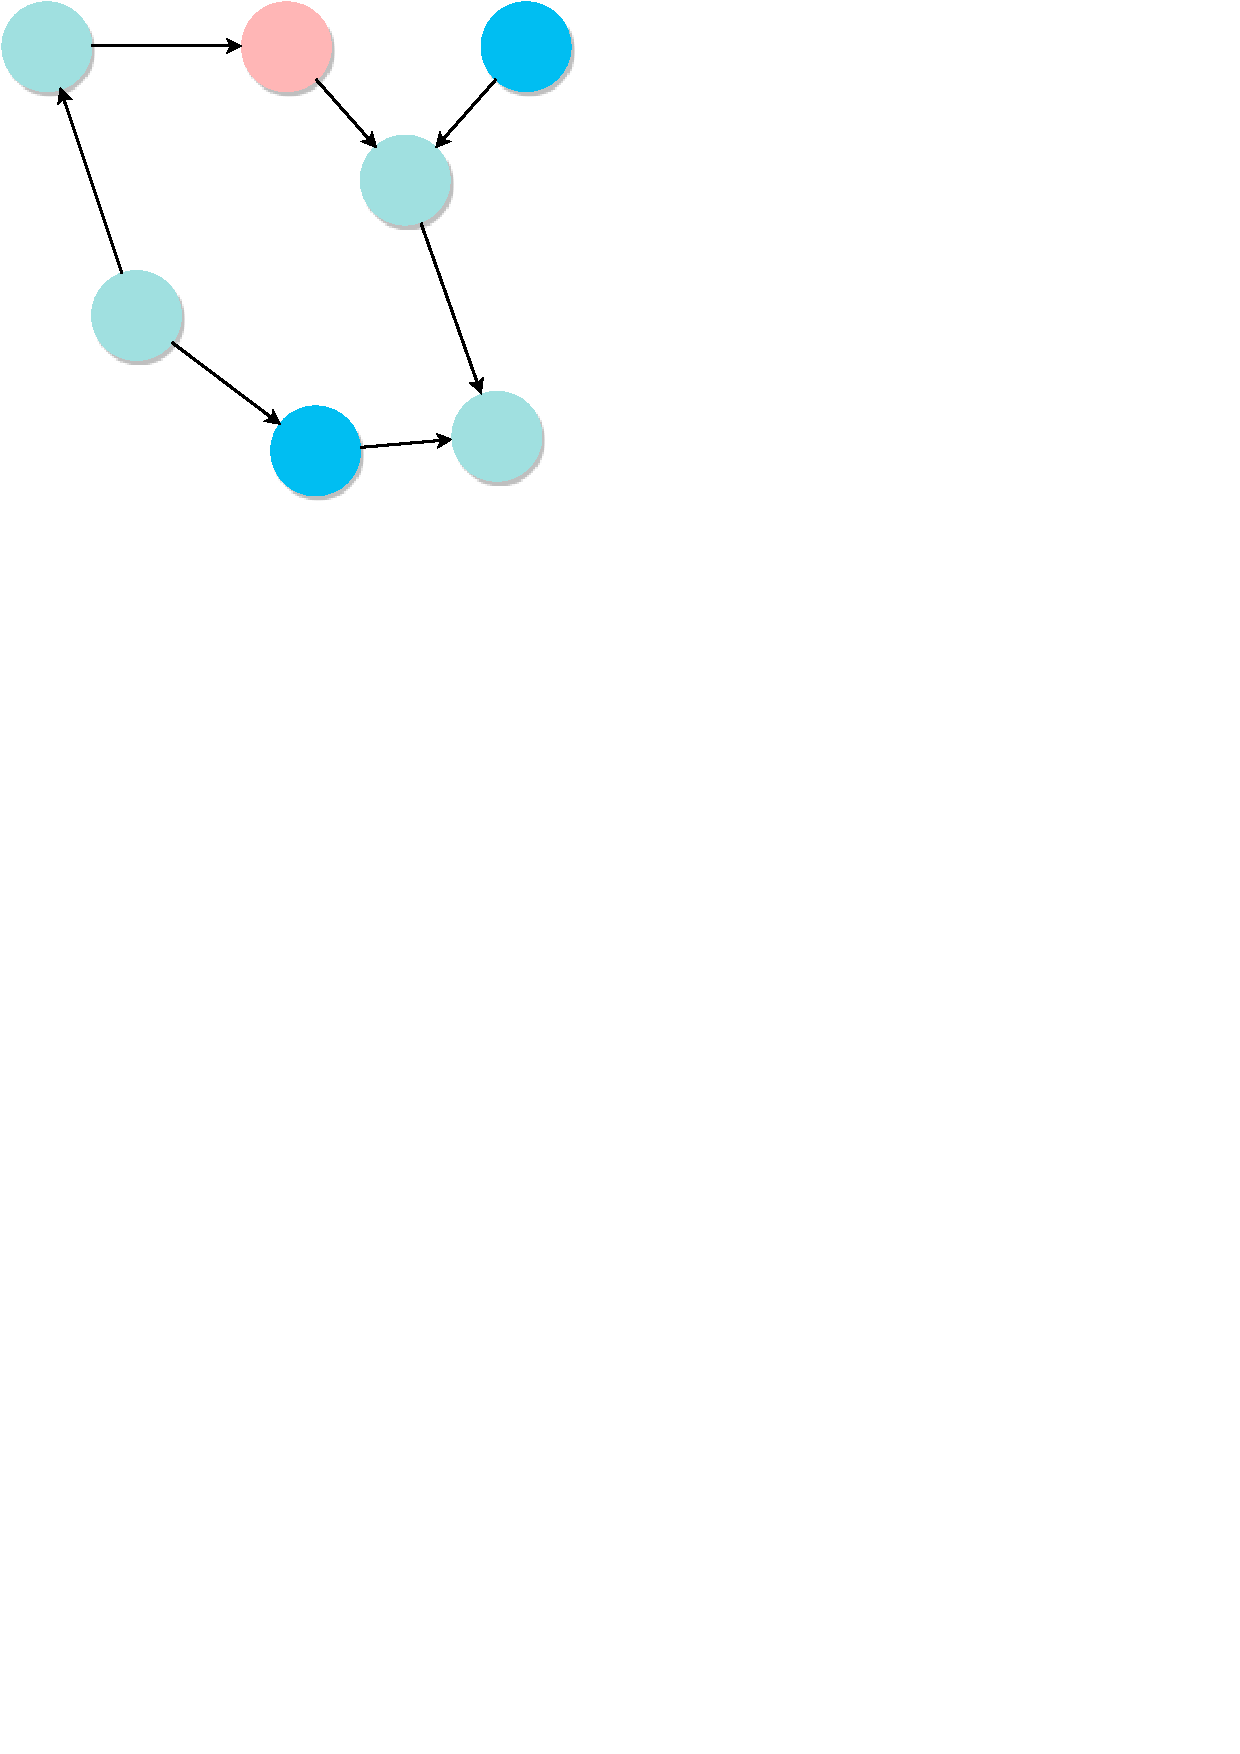
\includegraphics[trim=0 500 200 0,clip,width=0.5\textwidth]{images/motivation_left-1}}}
    \includegraphics<5>[trim=0 500 200 0,clip,width=0.5\textwidth]{images/motivation_left-2}
    \includegraphics<6>[trim=0 500 200 0,clip,width=0.5\textwidth]{images/motivation_left-3}
\end{figure}

\end{frame}


\begin{frame}{Goal}
\begin{block}{Goal}
Analytical queries on internal data \& external linked data
\end{block}
\pause
\begin{block}{Benefits}
\begin{itemize}
    \item Enables exploratory queries
    \item Increasing amount of linked data
    \item Integrates with heterogeneous data
    \item Semantic reasoning
\end{itemize}
\end{block}
\end{frame}

\begin{frame}{The First Steps}
\begin{block}{}
 Efficient Processing of Analytical Querying on RDF Data Cubes.
\end{block}
\pause
\begin{itemize}
    \item Denormalize the cube dimensions
    \item Reduce the subject-object joins (expensive)
    \item Increase the subject-subject joins
\end{itemize}
\begin{columns}
\column{0.5\textwidth}

\column{0.5\textwidth}
\begin{figure}
    
\includegraphics[width=\textwidth]{images/step-by-clip-art-849063.jpg}
\end{figure}
\end{columns}

\end{frame}

\begin{frame}{Workflow}

\begin{figure}
\centering
    \includegraphics<+>[trim=0 655 253 0,clip,height=0.7\textheight]{images/Workflow-3}
    \includegraphics<+>[trim=0 655 253 0,clip,height=0.7\textheight]{images/Workflow-4}
    \includegraphics<+>[trim=0 655 253 0,clip,height=0.7\textheight]{images/Workflow-5}
    \includegraphics<+>[trim=0 655 253 0,clip,height=0.7\textheight]{images/Workflow-6}
    \includegraphics<+>[trim=0 655 253 0,clip,height=0.7\textheight]{images/Workflow-7}
    \includegraphics<+>[trim=0 655 253 0,clip,height=0.7\textheight]{images/Workflow-8}
    \includegraphics<+>[trim=0 655 253 0,clip,height=0.7\textheight]{images/Workflow-9}
    \includegraphics<+->[trim=0 655 253 0,clip,height=0.7\textheight]{images/Workflow-10}
\end{figure}
\begin{itemize}
    \item<+-> Internal optimization 
\end{itemize}
\end{frame}

%\begin{frame}{Running Example}
%\begin{figure}
%    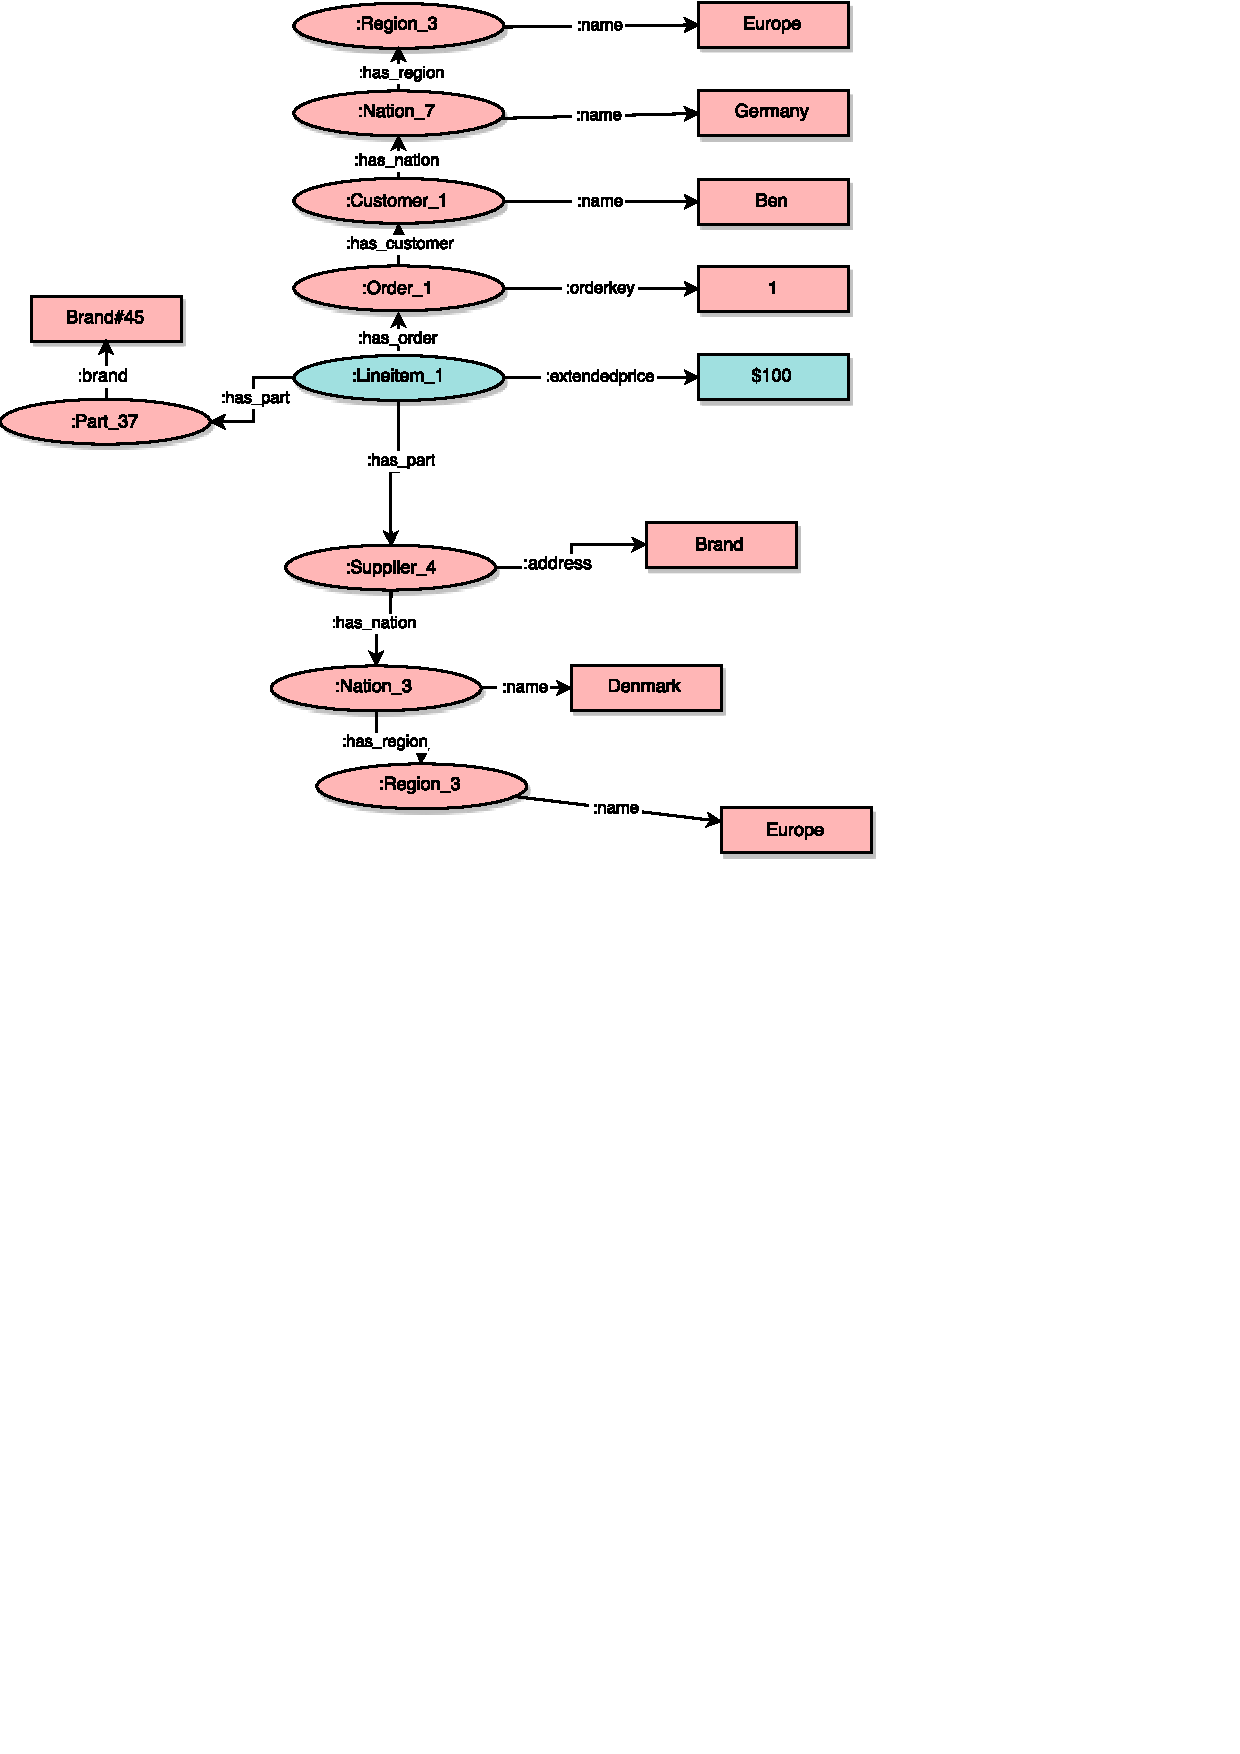
\includegraphics[trim=0 200 0 0,clip,width=\textwidth]{images/dataset_instance_example.pdf}
%\end{figure}
%\end{frame}

\begin{frame}{Building the Cube}
\begin{columns}
\column{0.5\textwidth}
\begin{block}{Purpose}
\begin{itemize}
    \item Organize data with purpose of analysis
    \item Easies to understand
\end{itemize}
\end{block}
\column{0.5\textwidth}
\begin{figure}
        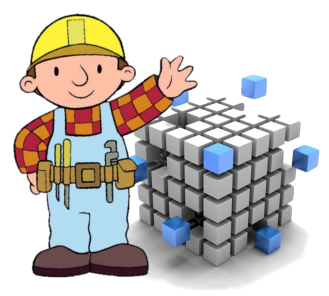
\includegraphics[width=0.8\textwidth]{images/cubeBuilder.png}
    \end{figure}
\end{columns}


\uncover<2>{
\begin{block}{What is a cube}
\begin{itemize}
    \item Facts: The subject of the analysis
    \item Dimensions: Perspectives of the data
    \item Levels: Concepts in the dimensions
\end{itemize}
\end{block}}
\end{frame}

\begin{frame}{\patsec}{Snowflake Pattern}
    \begin{figure}
        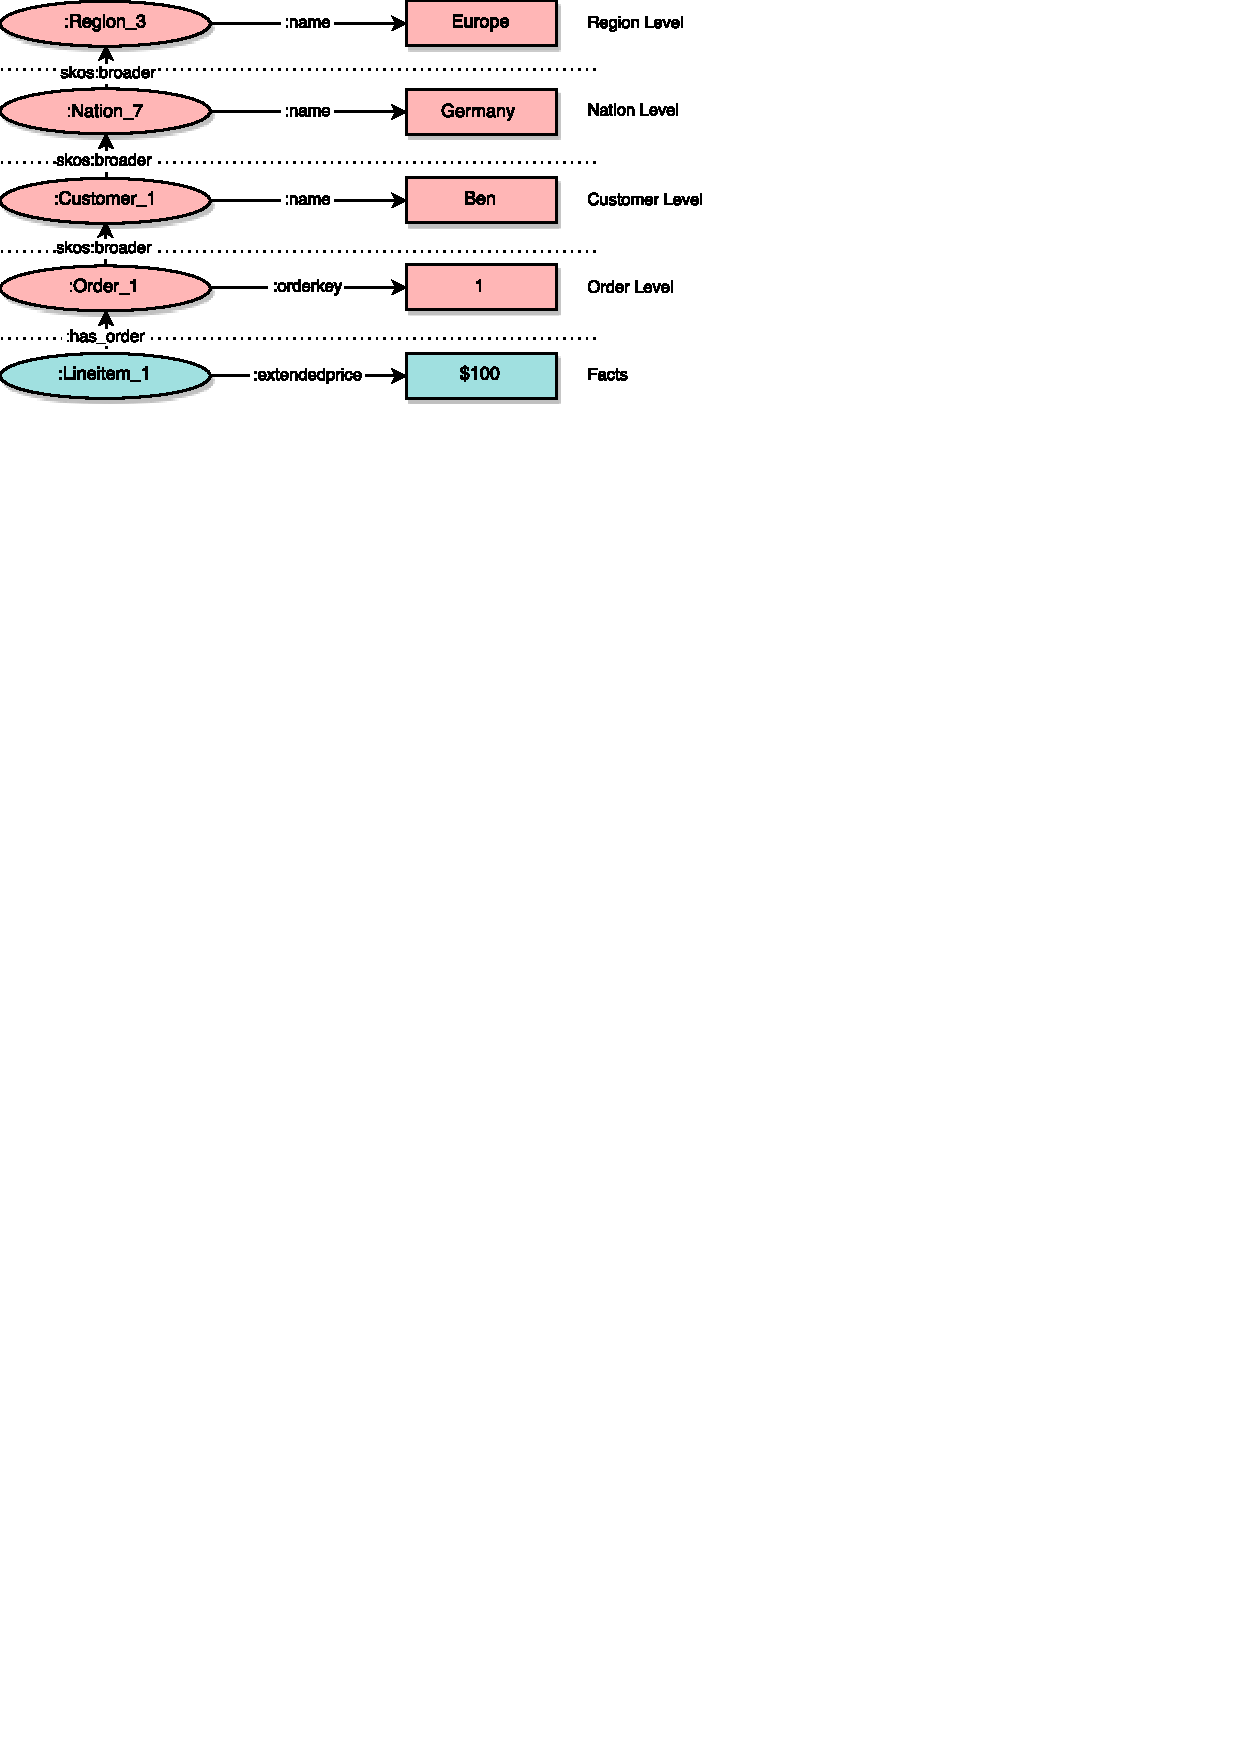
\includegraphics[trim=0 648 255 0,clip,width=1\textwidth]{images/snowflakepattern.pdf}
    \end{figure}
\end{frame}

%\begin{frame}{Requirements}
%\begin{columns}
%\column{.5\textwidth}
%\begin{block}{}
%\begin{itemize}
%    \item Observations
%    \item Level members
%    \item Relations between levels
%    \item Level attributes
%\end{itemize}
%\end{block}
%\column{.5\textwidth}
%    
%\end{columns}
%
%\begin{block}{Candidate Ontologies}
%\begin{itemize}
%    \item QB%\cite{dataCube}
%    \item QB4OLAP%\cite{DBLP:conf/semweb/EtcheverryV12}
%\end{itemize}
%\end{block}
%\end{frame}

\newcommand{\patsec}{Patterns}
\section{\patsec}
\begin{frame}{\patsec}{Star Pattern}
    \begin{figure}
        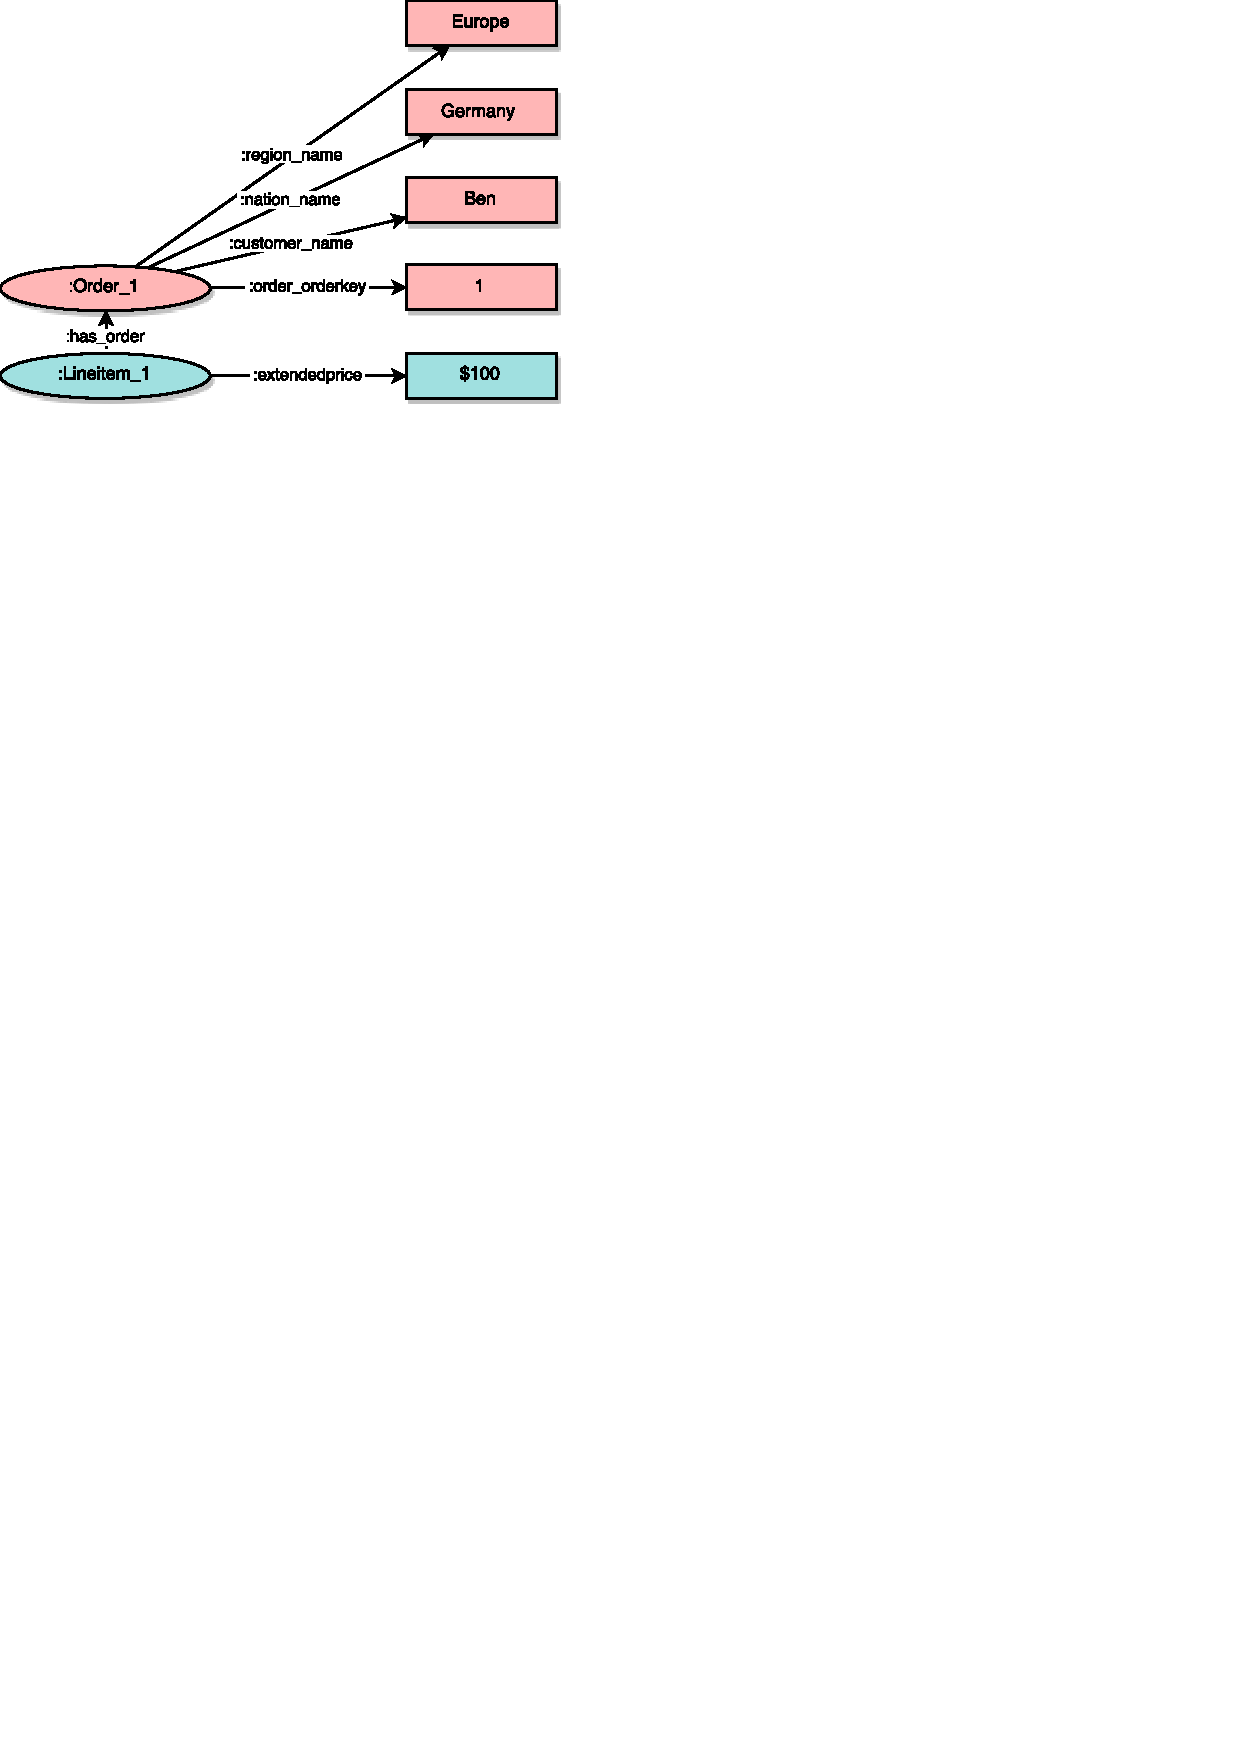
\includegraphics[trim=0 648 255 0,clip,width=1\textwidth]{images/starpattern.pdf}
    \end{figure}
\end{frame}

\begin{frame}{\patsec}{Denormalized Pattern}
    \begin{figure}
        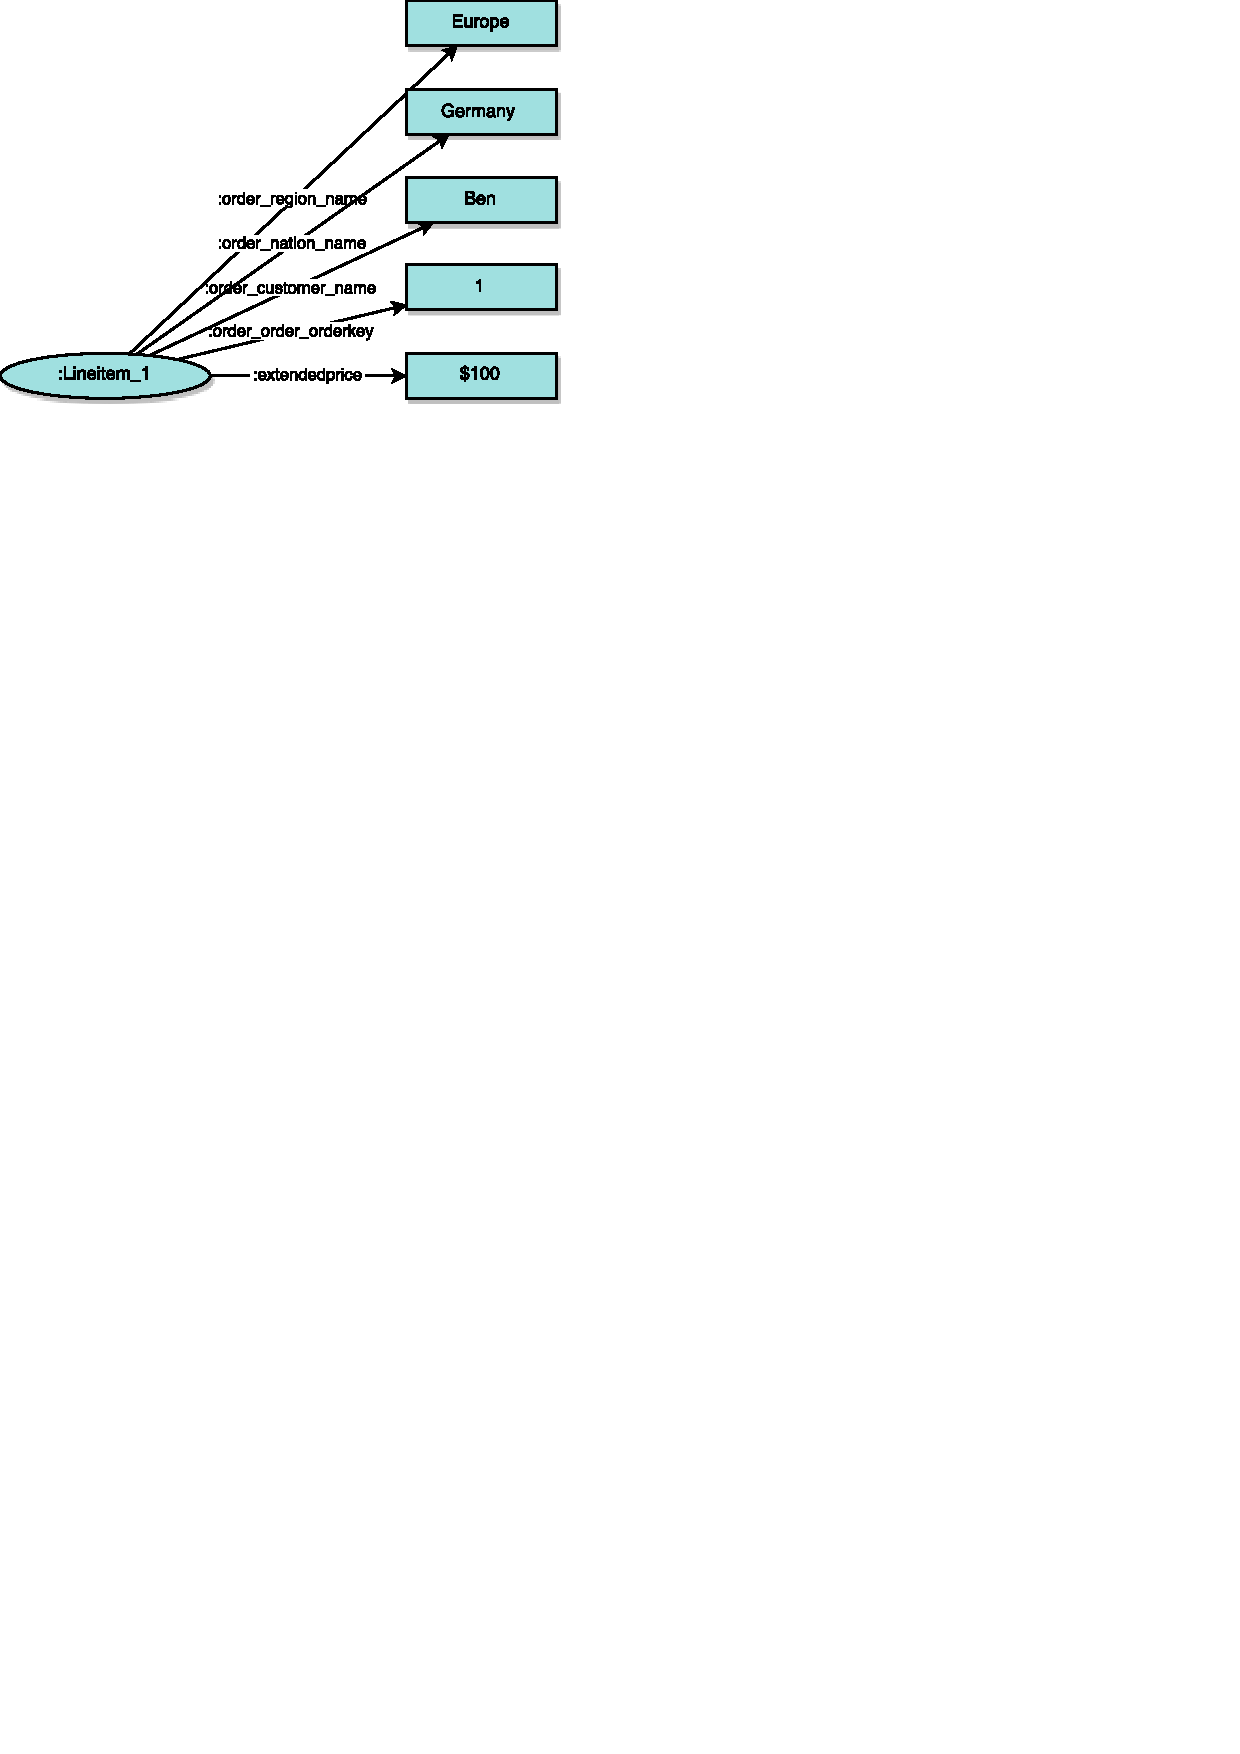
\includegraphics[trim=0 648 255 0,clip,width=1\textwidth]{images/denormalizedpattern.pdf}
    \end{figure}
\end{frame}

\section{SWOD}
\begin{frame}{Special Cases:}{Unbalanced Hierarchies}
\begin{figure}[tb]
    \begin{center}
        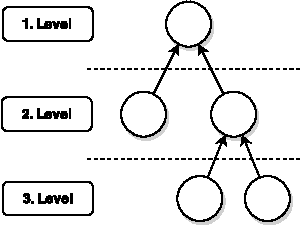
\includegraphics[width=0.8\textwidth]{images/alg-unbal-abstract-base}
    \end{center}
\end{figure}
\end{frame}


\begin{frame}{Special Cases:}{Property Collision}
    \begin{figure}
        \includegraphics<+>[trim=0 648 255 0,clip,width=1\textwidth]{images/property_collision-0.pdf}
        \includegraphics<+>[trim=0 648 255 0,clip,width=1\textwidth]{images/property_collision-1.pdf}
        \includegraphics<+>[trim=0 648 255 0,clip,width=1\textwidth]{images/property_collision-2.pdf}
    \end{figure}
\end{frame}


\begin{frame}{Semantic Web OLAP Denormalization Algorithm}
\begin{columns}
    \column{0.5\textwidth}
    \begin{block}{Input}
        \begin{itemize}
            \item QB4OLAP ontology
            \item Snowflake pattern RDF data cube
        \end{itemize}
    \end{block}

    \begin{block}{Output}
        \begin{itemize}
            \item Star pattern RDF data cube
            \item Fully Denormalized pattern RDF data cube
        \end{itemize}
    \end{block}

    \begin{block}{Features}
        \begin{itemize}
            \item Top-down traversal
            \item Property renaming
        \end{itemize}
    \end{block}

    
    \column{0.5\textwidth}
    \begin{figure}
        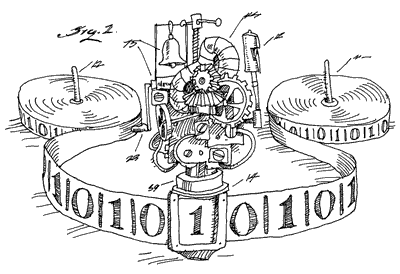
\includegraphics[width=\textwidth]{images/turingMachine.png}
    \end{figure}    
\end{columns}
\end{frame}


\begin{frame}{Unbalanced Hierarchies Example}
\begin{figure}
    \includegraphics<+>[trim=0 648 145 0,clip,width=1\textwidth]{images/unbalanced_hierarchies-a.pdf}
    \includegraphics<+>[trim=0 648 145 0,clip,width=1\textwidth]{images/unbalanced_hierarchies-b.pdf}
    \includegraphics<+>[trim=0 648 145 0,clip,width=1\textwidth]{images/unbalanced_hierarchies-c.pdf}
    \includegraphics<+>[trim=0 648 145 0,clip,width=1\textwidth]{images/unbalanced_hierarchies-d.pdf}
    \includegraphics<+>[trim=0 648 145 0,clip,width=1\textwidth]{images/unbalanced_hierarchies-e.pdf}
    \includegraphics<+>[trim=0 648 145 0,clip,width=1\textwidth]{images/unbalanced_hierarchies-f.pdf}
\end{figure}
\end{frame}

\begin{frame}[fragile]{Query rewriting}
\begin{columns}
\column{0.5\textwidth}
\begin{lstlisting}[style=rdf, captionpos=b,label=lst:snow, basicstyle=\scriptsize]
SELECT ?name sum(?price)
WHERE {
 ?lineitem :extendedprice ?price;
           :has_order ?order .
 ?order skos:broader ?customer .
 ?customer skos:broader ?nation .
 ?nation :name ?name .
}
GROUP BY ?name
\end{lstlisting}
\column{0.5\textwidth}
\end{columns}

\begin{columns}
\column{0.5\textwidth}
\centering
\begin{figure}
    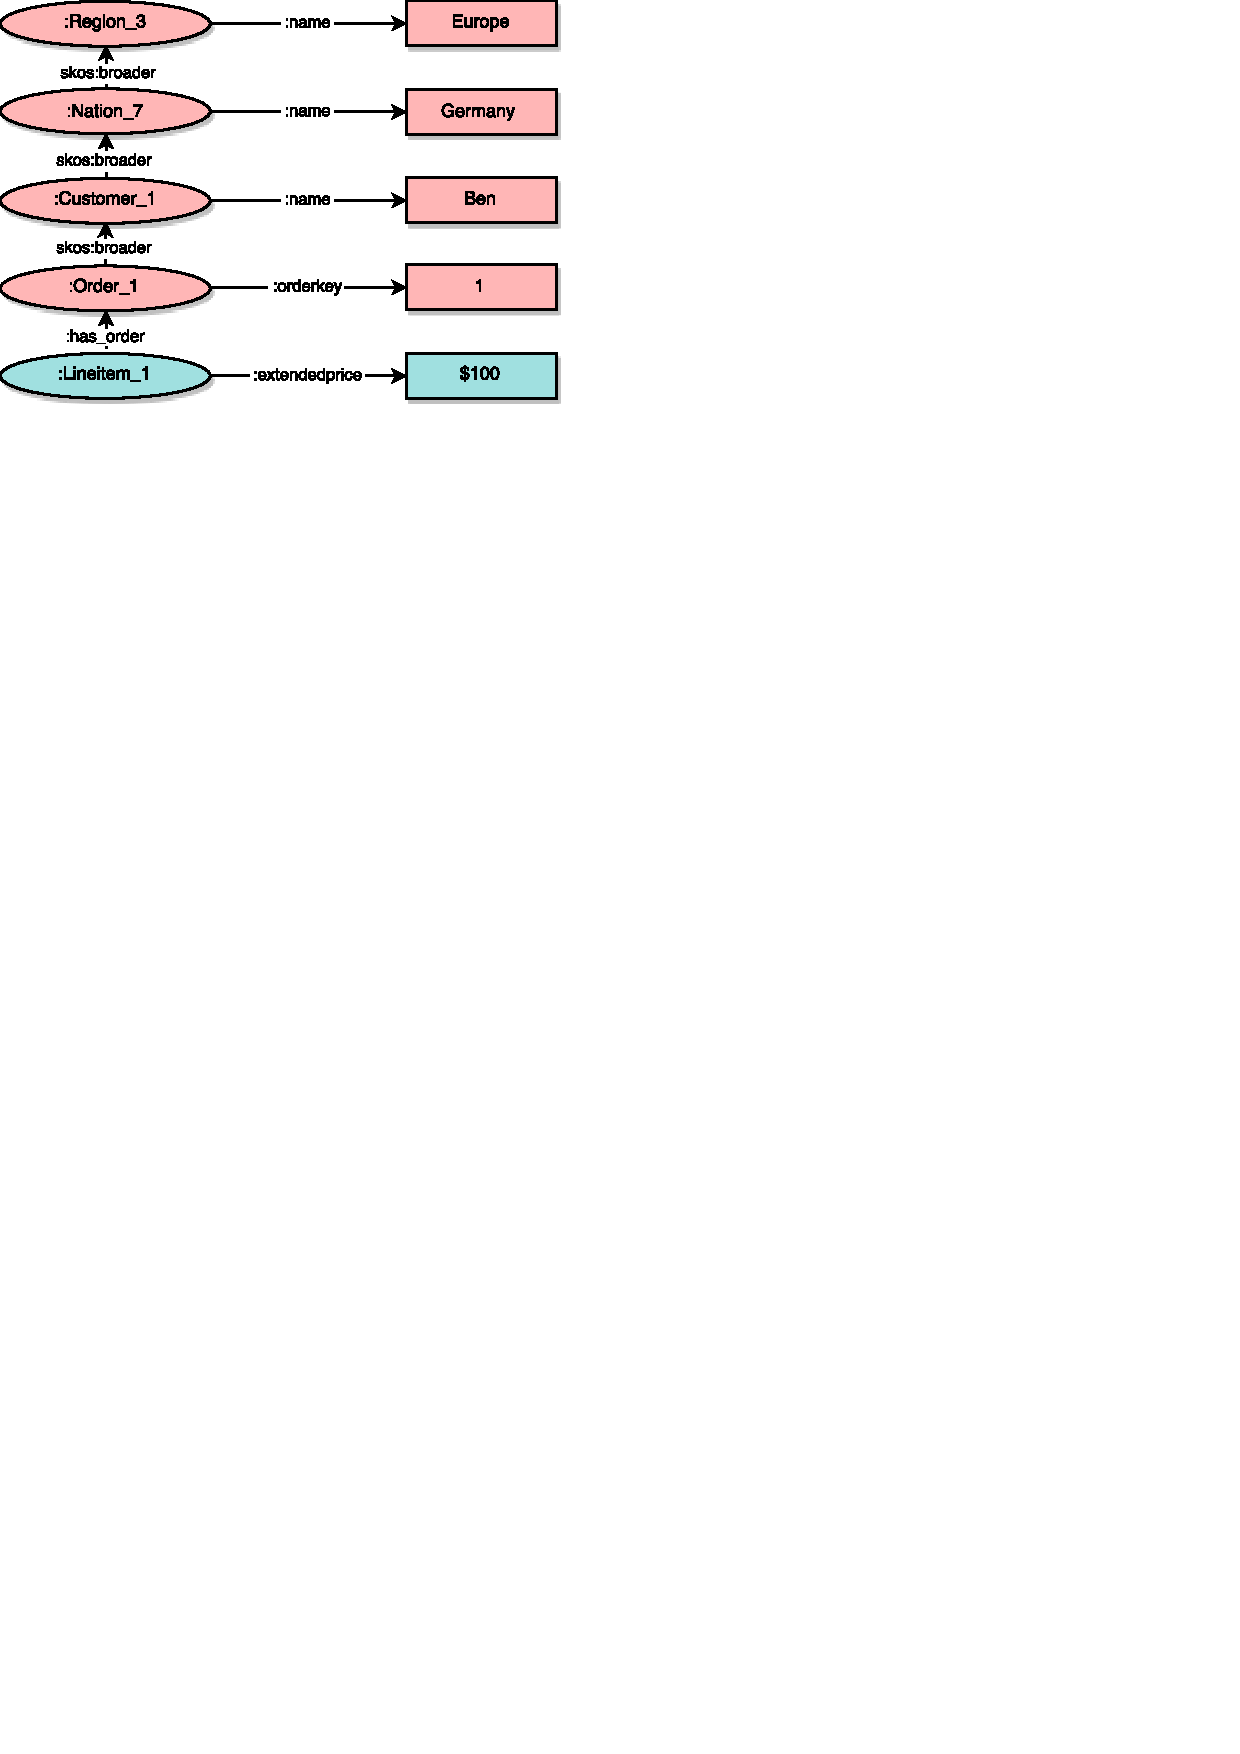
\includegraphics[trim=0 648 280 0,clip,width=1\textwidth]{images/snowflakepattern-0.pdf}
\end{figure}
\column{0.5\textwidth}
\end{columns}
\end{frame}


\begin{frame}[fragile]{Query rewriting}
\begin{columns}
\column{0.5\textwidth}
\begin{lstlisting}[style=rdf, captionpos=b,label=lst:snow, basicstyle=\scriptsize]
SELECT ?name sum(?price)
WHERE {
 ?lineitem :extendedprice ?price;
           :has_order ?order .
 ?order skos:broader ?customer .
 ?customer skos:broader ?nation .
 ?nation :name ?name .
}
GROUP BY ?name
\end{lstlisting}
\column{0.5\textwidth}
\begin{lstlisting}[style=rdf, captionpos=b, label=lst:star, basicstyle=\scriptsize]
SELECT ?name sum(?price)
WHERE {
 ?lineitem :extendedprice ?price;
           :has_order ?order .
 ?order :nation_name ?name .
}
GROUP BY ?name
\end{lstlisting}
\end{columns}

\begin{columns}
\column{0.5\textwidth}
\centering
\begin{figure}
    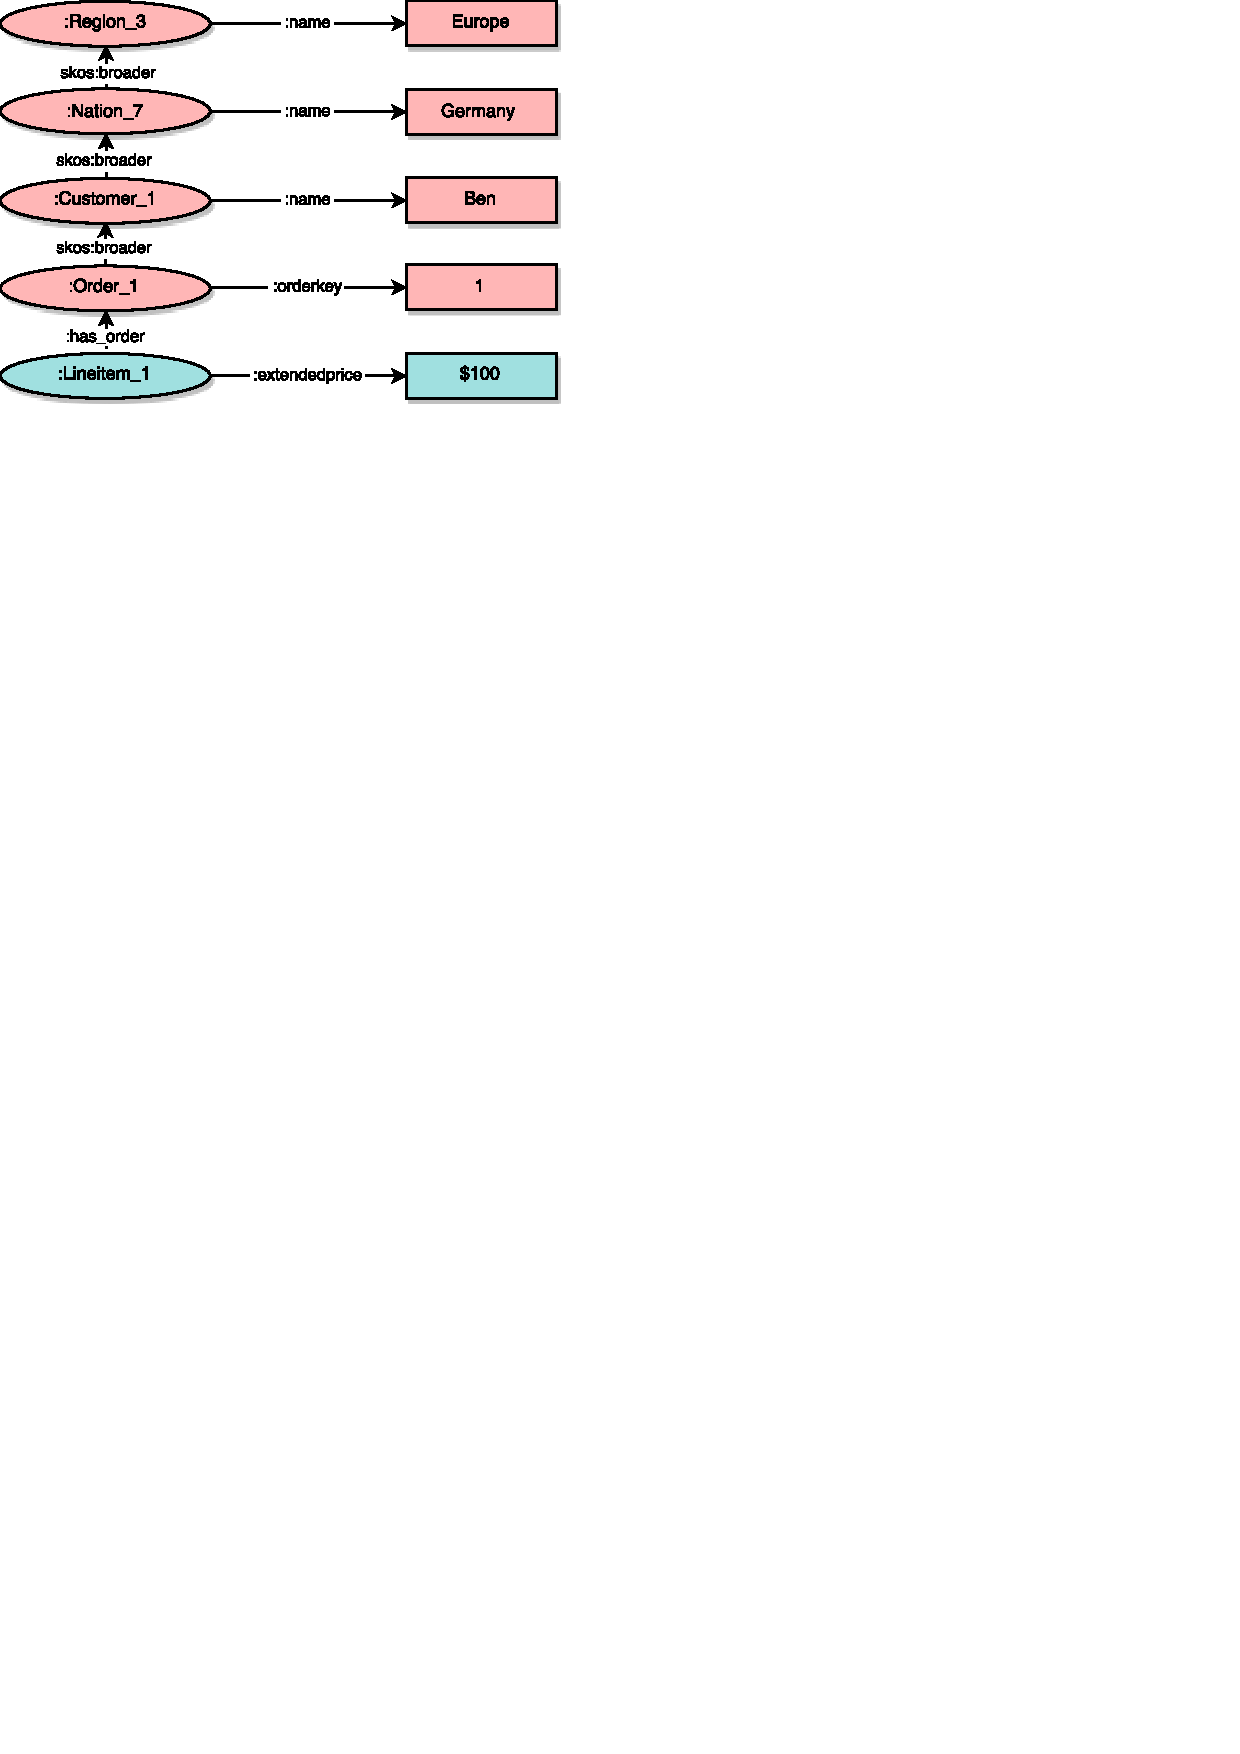
\includegraphics[trim=0 648 280 0,clip,width=1\textwidth]{images/snowflakepattern-0.pdf}
\end{figure}
\column{0.5\textwidth}
\centering
\begin{figure}
    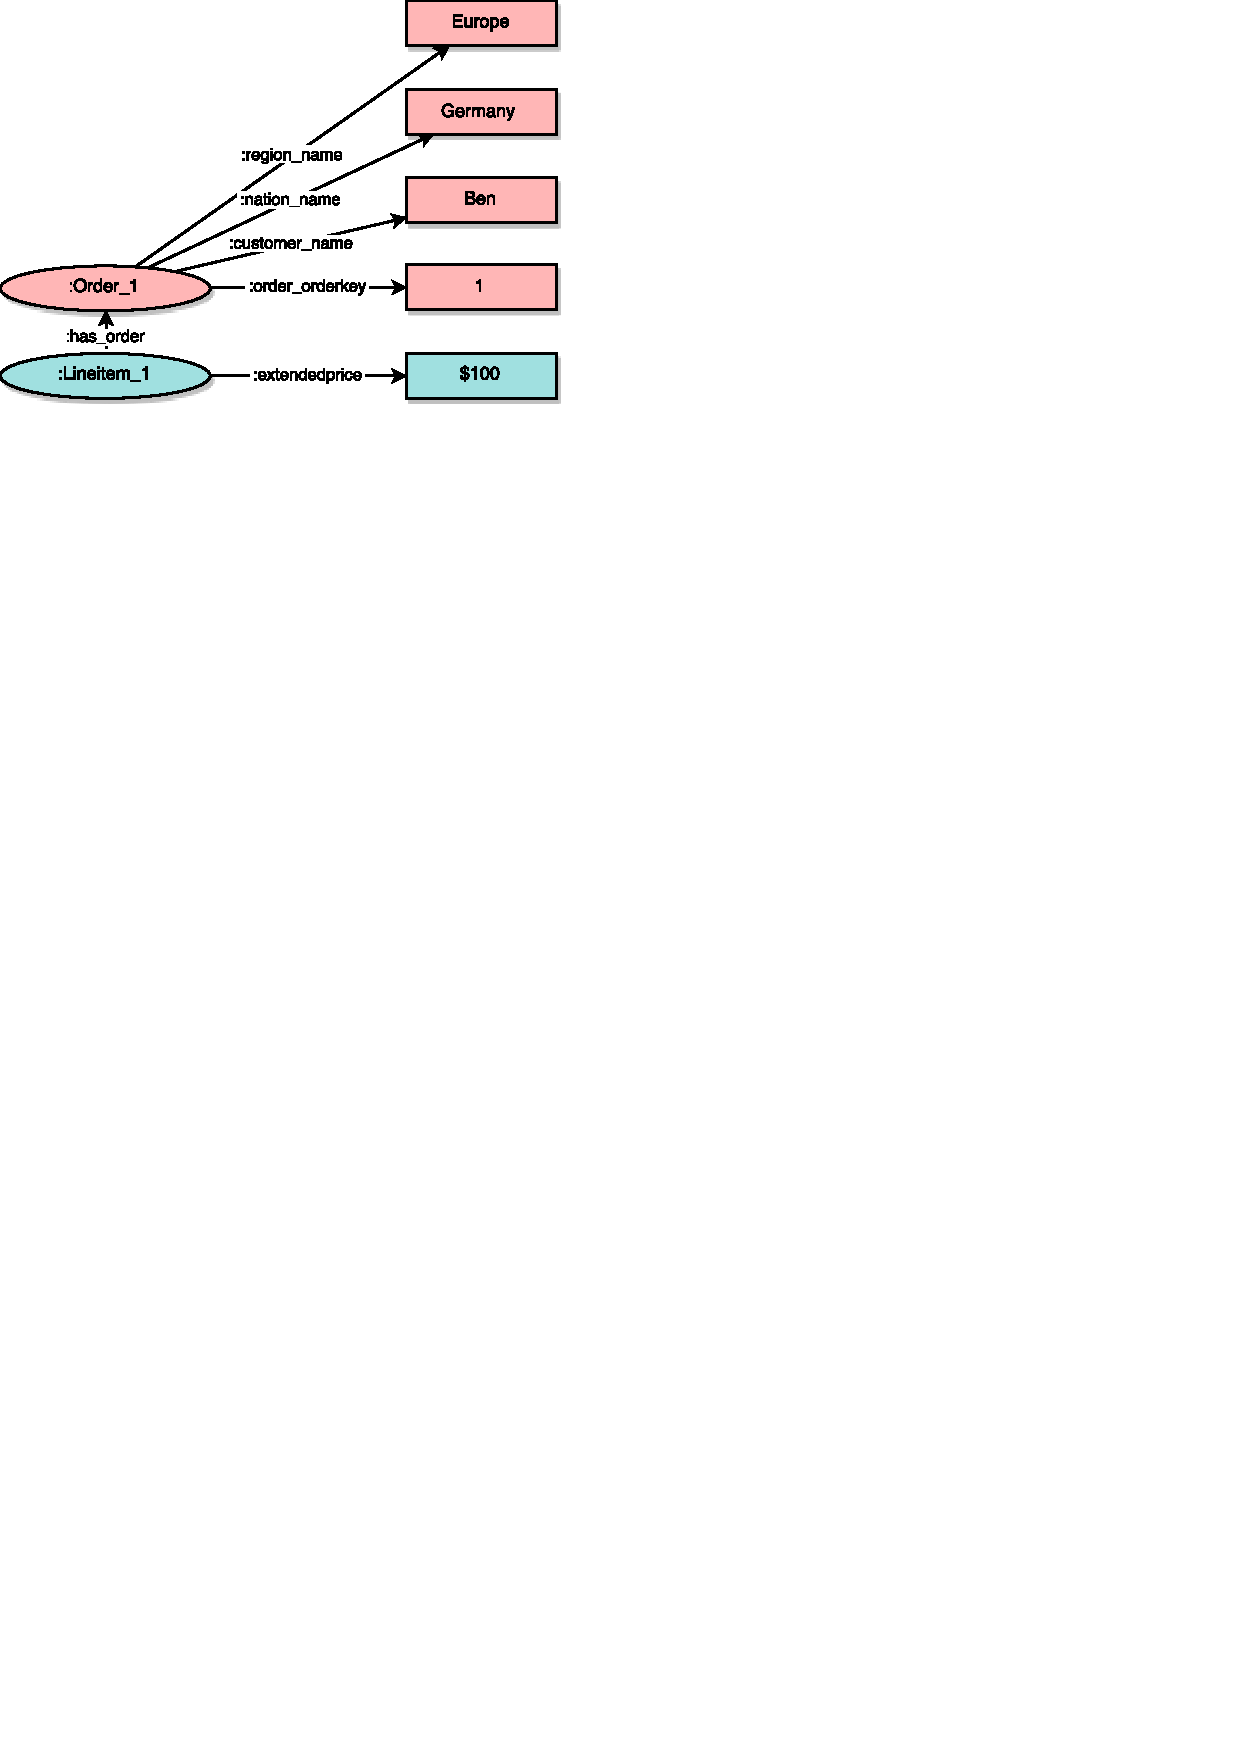
\includegraphics[trim=0 648 280 0,clip,width=1\textwidth]{images/starpattern.pdf}
\end{figure}
\end{columns}
\end{frame}

\section{Evaluation}
\begin{frame}{Results}
\begin{table}
    \begin{tabular}{l|r|r}
    \hline
    \multicolumn{3}{c}{Virtuoso} \\ \hline
    ~        & Star & Denormalized \\ \hline
    Increase in Triples  & 16 \%     & 173 \%       \\
    Avg. Decease in Query Time     & 600 \%    & 700 \%       \\
    Geo. M. Decease in Query Time & 110 \%    & 140 \%       \\
    \end{tabular}
\end{table}
\begin{itemize}
    \item Cost of triple storage
    \item Static and frequently changing data
\end{itemize}
\end{frame}




\newcommand{\conc}{Future Work}
\begin{frame}{\conc}
\begin{columns}
\column{0.5\textwidth}
\begin{itemize}
    \item More cube optimizations
    \item Consider data provenance and quality
\end{itemize}
\column{0.5\textwidth}
\begin{figure}

\includegraphics[width=\textwidth]{images/The-present-of-work.jpg}
\end{figure}
\end{columns}


\end{frame}

%\setbeamertemplate{headline}{}
\begin{frame}[plain]{}
\centering
\Huge{Thank you}
\end{frame}



%\begin{frame}[allowframebreaks,noframenumbering]
%        \frametitle{References}
%        \bibliographystyle{amsalpha}
%        \bibliography{references.bib}
%\end{frame}


\begin{frame}[noframenumbering]{SWOD Abstract}
\framesubtitle{Example}
\begin{figure}[]
  \centering
  \includegraphics<+>[height=0.8\textheight]{images/00-SWOD.pdf}
  \includegraphics<+>[height=0.8\textheight]{images/0-SWOD.pdf}
  \includegraphics<+>[height=0.8\textheight]{images/1-SWOD.pdf}
  \includegraphics<+>[height=0.8\textheight]{images/2-SWOD.pdf}
  \includegraphics<+>[height=0.8\textheight]{images/3-SWOD.pdf}
  \includegraphics<+>[height=0.8\textheight]{images/5-SWOD.pdf}
  \includegraphics<+>[height=0.8\textheight]{images/6-SWOD.pdf}
  \includegraphics<+>[height=0.8\textheight]{images/7-SWOD.pdf}
  \includegraphics<+>[height=0.8\textheight]{images/8-SWOD.pdf}
  \includegraphics<+>[height=0.8\textheight]{images/9-SWOD.pdf}
  \includegraphics<+>[height=0.8\textheight]{images/10-SWOD.pdf}
  \includegraphics<+>[height=0.8\textheight]{images/11-SWOD.pdf}
  \includegraphics<+>[height=0.8\textheight]{images/12-SWOD.pdf}
\end{figure}
\end{frame}

\begin{frame}[noframenumbering]{Figure Credits}
\begin{itemize}
    \item Workman -- Licence: CC BY 3.0 \\ Credit: www.clipartbest.com
    \item Cube -- Licence: CC BY 3.0 \\ Credit: www.clipartbest.com
    \item Turing machine \\ http://www.felienne.com/
    \item Steps \\ http://www.cliparthut.com/
    \item Future-work \\ http://www.horsesforsources.com/
\end{itemize}
\end{frame}



\end{document}